\section{\textit{Embeddings}}

El primer enfoque con el que se abordó el problema de clasificación propuesto para este taller consistió en construir los \textit{embeddings} (representaciones vectoriales de las palabras) con un modelo de Word2Vec. Este modelo utiliza una red neuronal para aprender las asociaciones de palabras a partir de un corpus de documentos o sentencias. Esto lo hace tratando de resolver la tarea de predecir la probabilidad de una palabra a partir de sus vecinos, el objetivo como tal no es resolver la tarea, sino aprender los pesos de la red, los cuales se convertirán en los vectores. \\

Para esto se utilizó la implementación de Word2Vec de la librería de \texttt{gensim}. A continuación se explican algunos de los parámetros clave para el entrenamiento del modelo y los valores que se definieron:

\begin{itemize}
    \item Tamaño del Embedding (\textit{embedding\_size}): La dimensionalidad del vector resultante como represesntación de cada uno de los términos. Se decidió realizar pruebas con 3 tipos de tamaños: pequeño (dim=15), mediano (dim=75) y grande (dim=150).
    
    \item Window: Ventana de tamaño que utiliza el modelo para considerar las palabras similares entre sí. En este caso se experimento con varios tamaños desde 1 hasta 10. Los mejores resultados para este parámetro se obtuvieron entre 2 y 3. Es decir, el modelo tiene en cuenta 2-3 palabras antes y 2-3 palabras después de la palabra que se trata de predecir.
    
    \item Min Count: Frecuencia mínima que debe tener una palabra para considerarla dentro del modelo, esto elimina términos extraños y muy poco frecuentes (puede ayudar con el sobreajuste u \textit{overffiting}). Se definió en 10, lo que redujo considerablemente el tamaño del vocabulario.
    
    \begin{figure}[H]
        \centering
        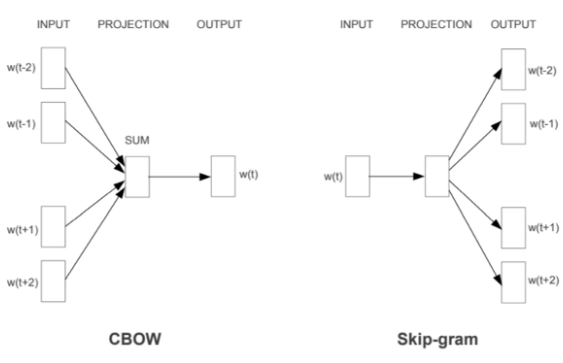
\includegraphics[scale=0.72]{doc/images/cbow_skipgram.png}
        \caption{Representación gráfica de los modelos de \textit{cbow} y \textit{skipgram}}
        \label{fig:cbow_skipgram}
    \end{figure}
    
    \item SG: Si utilizar un modelo de \textit{skipgram} o \textit{cbow}. Dos formas de implementar la tarea de predicción con la que se construyen los \textit{embeddings} (véase figura \ref{fig:cbow_skipgram}). La primera usa la representación de la palabra de entrada para predecir el contexto y la segunda utiliza la representación del contexto para predecir la palabra. Para esta tarea se utilizó el modelo \textit{cbow.}
    
    \item Negative: El número de palabras (seleccionadas al azar o \textit{sampled}) utilizadas como ejemplo negativo al momento de entrenar el modelo.
    
\end{itemize}

\subsection{2D Plots}

Dado el tamaño de los \textit{embeddings} (15, 75 y 150), se utiliza una técnica de reducción de dimensionalidad para poder visualizar algunos de los términos (vectores) interesantes y sus relaciones en un plano 2D. En este caso, se decidió utilizar la técnica de Análisis de Componentes Principales (o PCA por sus siglas en inglés). Esta técnica hace una transformación lineal de los datos y los proyecta sobre un nuevo eje coordenado, buscando preservar la mayor varianza (información explicativa del vector) en cada uno de sus ejes. De aquí su nombre de Componentes Principales, pues se trabaja con las bases (componentes) que contiene la mayor variabilidad de los datos (principales). \\

Así las cosas, a continuación se presentan los personajes principales de cada una de las series y las palabras más similares a estos (a nivel vectorial) proyectados en un plano 2D.

\subsubsection{Simpsons Dataset}

En la figura \ref{fig:simpsons_sim_words} se puede observar que sin importar el tamaño del \textit{embedding}, todos los modelos de Word2Vec muestran una alta similitud entre los personajes principales. Esto pues en todos los casos se observa que las palabras más similares siempre incluyen a los otros personajes principales. Esto tiene sentido, pues teniendo en cuenta el funcionamiento de Word2Vec y que el \textit{dataset} con el que se está trabajando corresponde a las líneas de dialogo, las palabras más similares serán aquellas que acompañen comúnmente a la palabra del personaje. \\

Ahora bien, dado que es recurrente que los personajes principales estén juntos, es común que se refieran a varios de ellos en la misma frase. No obstante, hay algunas relaciones interesantes que vale la pena mencionar: 

\begin{itemize}
    \item El carácter \textit{j}, asociado al segundo nombre de Homero (Homer J. Simpson) para los embeddings de tamaño 75 y 150.
    
    \item Personajes como Nelson y Milhouse similares a Lisa y Bart.
    
    \item Términos cariñosos como \textit{honey}, \textit{sweetie} y \textit{homie} especialmente relacionados con Marge y Lisa.
    
    \item Términos como papá, mamá e hijo (\textit{dad, mom, son}) cercanos a varios de los personajes.
\end{itemize}

\begin{figure}[H]

\centering
\begin{minipage}{0.47\textwidth}
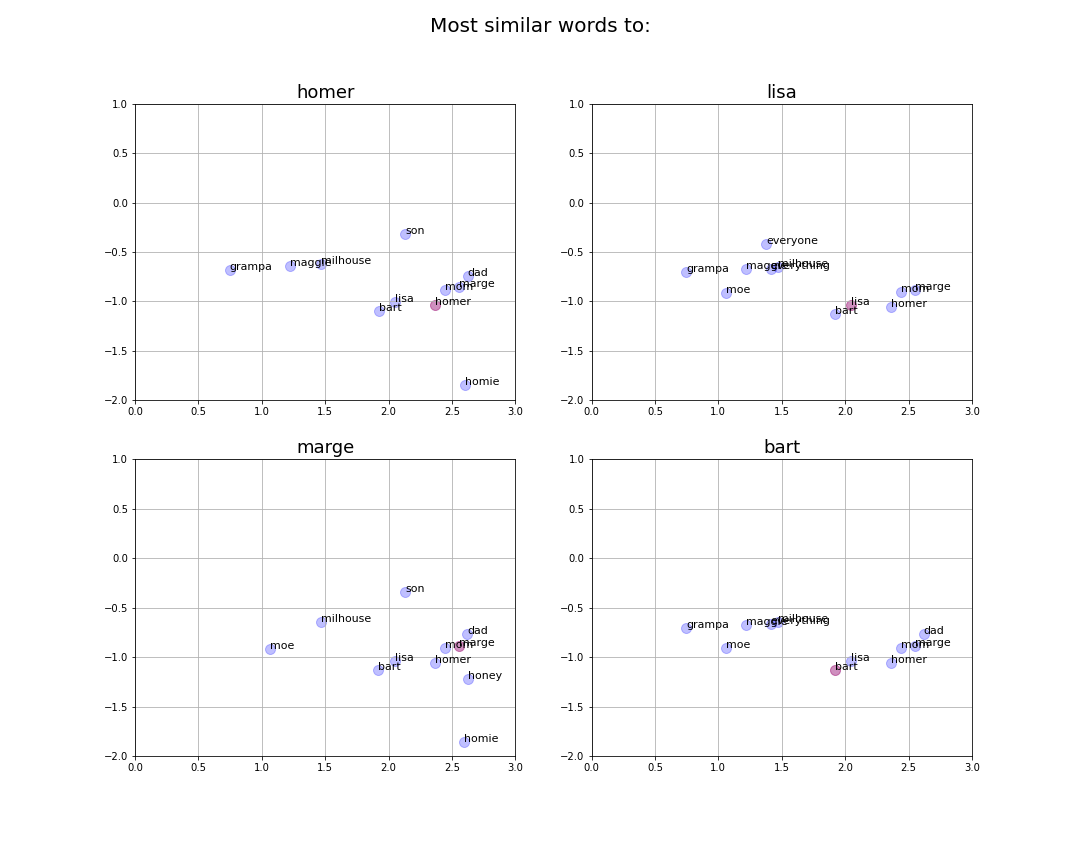
\includegraphics[trim=4.2cm 3cm 3.7cm 2.7cm, clip=true, width=\textwidth]{results/embeddings/simpsons_similar_15.png}
\caption*{a) DIM = 15}
\end{minipage}\hfill
\begin{minipage}{0.47\textwidth}
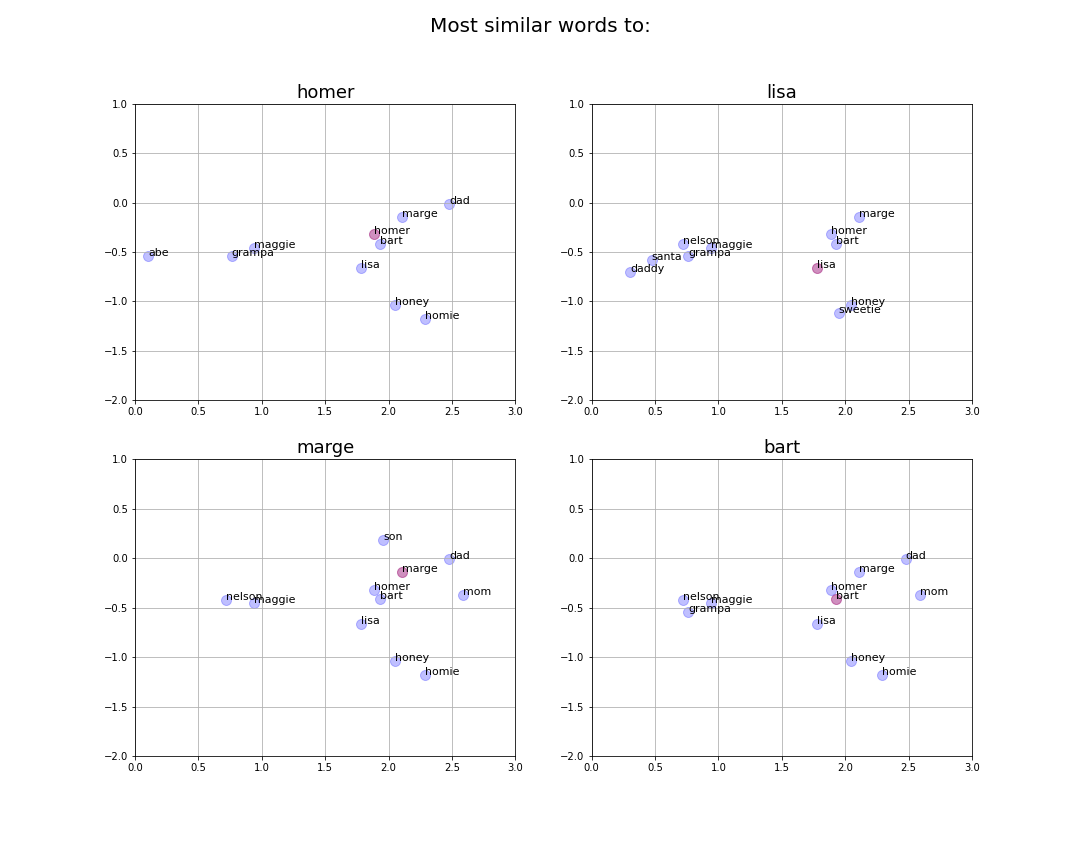
\includegraphics[trim=4.2cm 3cm 3.7cm 2.7cm, clip=true, width=\textwidth]{results/embeddings/simpsons_similar_75.png}
\caption*{b) DIM = 75}
\end{minipage}\par
\vskip\floatsep% normal separation between figures
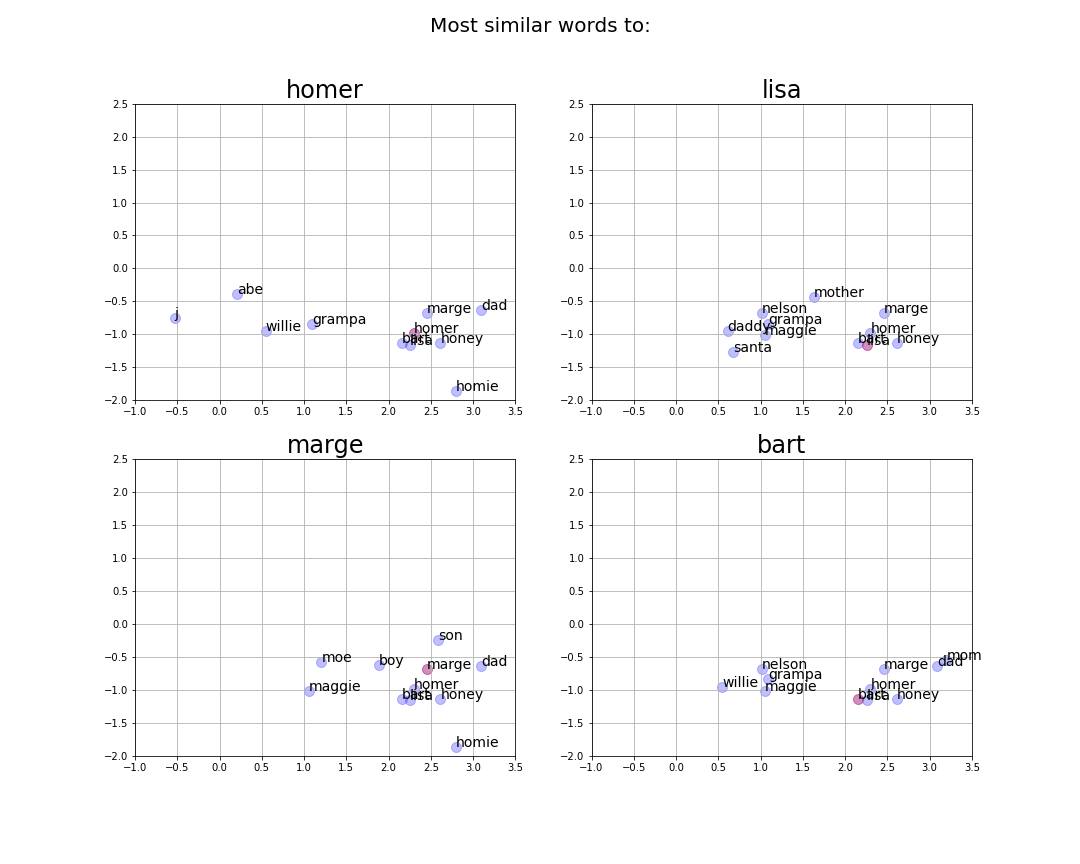
\includegraphics[trim=4.2cm 3cm 3.7cm 2.7cm, clip=true, width=0.45\textwidth]{results/embeddings/simpsons_similar_150.png}
\caption*{c) DIM = 150}
\caption{\textit{Embeddings} de los personajes principales de los \textbf{\textit{Simpsons}} y los términos más similares proyectados en un plano 2D para distintos tamaño de \textit{embedding}}
\label{fig:simpsons_sim_words}

\end{figure}


\subsubsection{Friends Dataset}

Similar a los \textit{embeddings} del \textit{dataset} de los Simpsons se obtiene que los términos más similares a los personajes, son los otros personajes. No obstante, también se encuentran algunas relaciones interesantes:

\begin{itemize}
    \item Aparecen otros personajes como Gunther y Janice,
    
    \item Emma (la hija de Rachel y Ross) suele estar siempre relacionada a estos dos personajes.
    
    \item Pronombres masculinos como \textit{him}, relacionados sobretodo con los hombres.
\end{itemize}

\begin{figure}[H]

\centering
\begin{minipage}{0.47\textwidth}
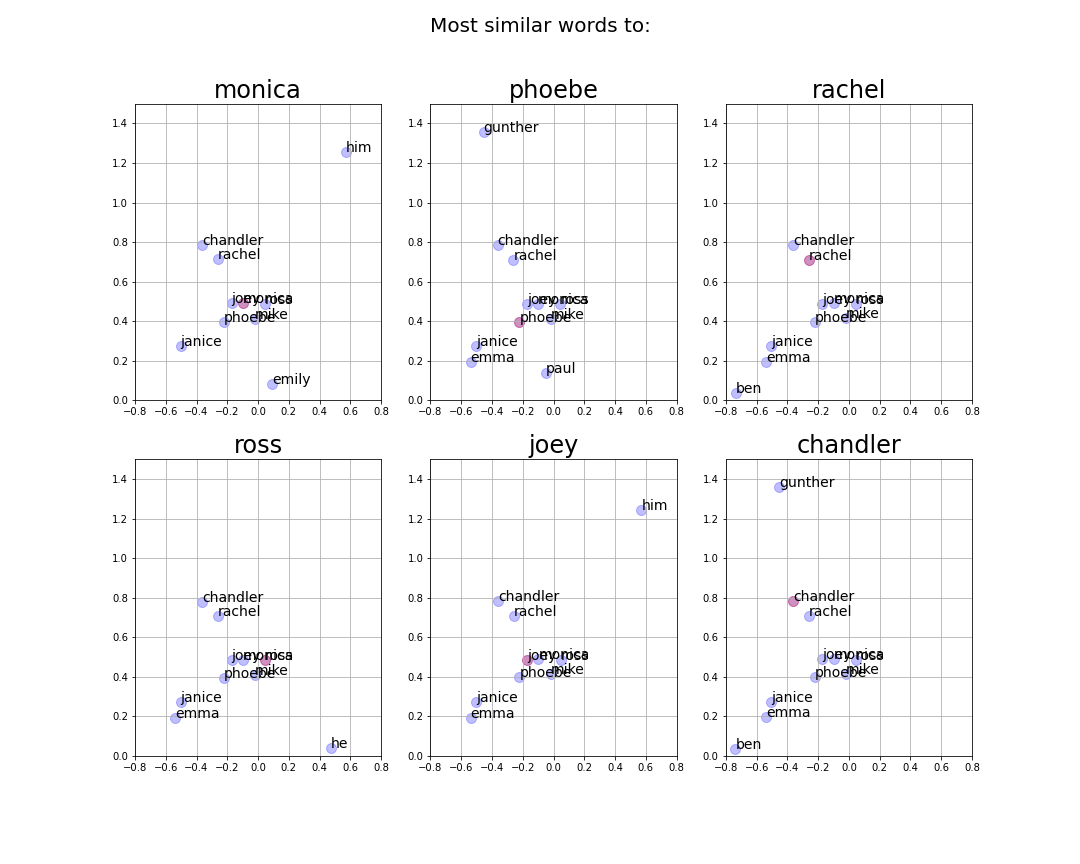
\includegraphics[trim=4.2cm 3cm 3.7cm 2.7cm, clip=true, width=\textwidth]{results/embeddings/friends_similar_15.png}
\caption*{a) DIM = 15}
\end{minipage}\hfill
\begin{minipage}{0.47\textwidth}
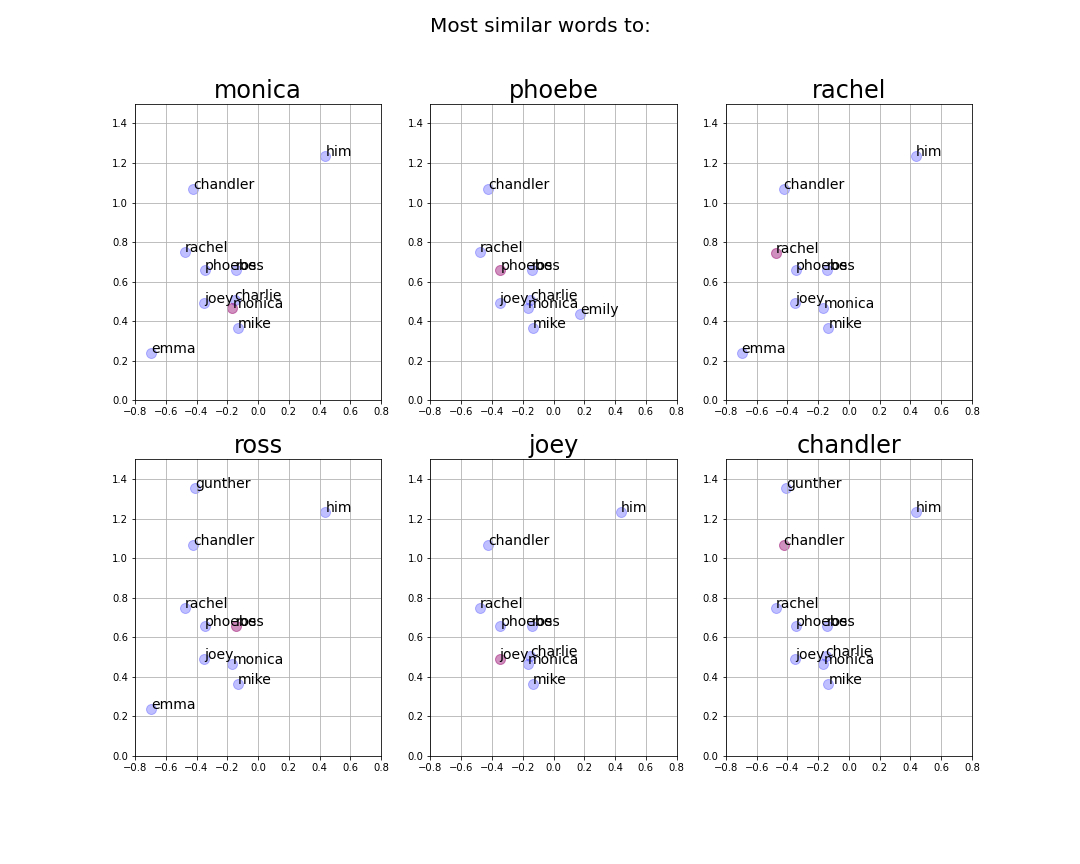
\includegraphics[trim=4.2cm 3cm 3.7cm 2.7cm, clip=true, width=\textwidth]{results/embeddings/friends_similar_75.png}
\caption*{b) DIM = 75}
\end{minipage}\par
\vskip\floatsep% normal separation between figures
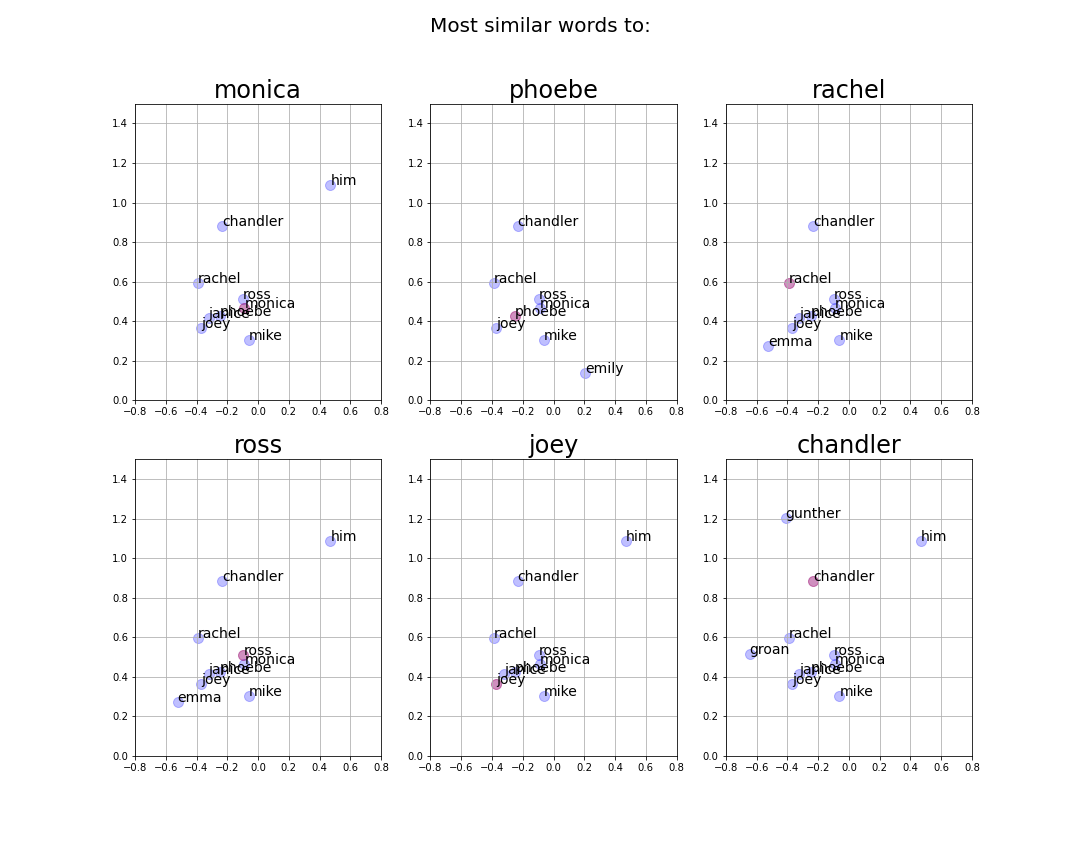
\includegraphics[trim=4.2cm 3cm 3.7cm 2.7cm, clip=true, width=0.45\textwidth]{results/embeddings/friends_similar_150.png}
\caption*{c) DIM = 150}
\caption{\textit{Embeddings} de los personajes principales de \textbf{\textit{Friends}} y los términos más similares proyectados en un plano 2D para distintos tamaño de embedding}
\label{fig:friends_sim_words}

\end{figure}

\subsection{Relaciones interesantes}

Finalmente, una de características principales y bastante interesantes de los \textit{embeddings} es que logran capturar la relación semántica de las palabras en un espacio vectorial. Razón por la cual los términos se pueden operar y se pueden encontrar algunas relaciones bastante interesantes. A partir de los modelos de word2vec, construidos en esta sección, se realizaron y analizaron algunas de las relaciones que surgieron en tres niveles diferentes:

\begin{itemize}
    \item \textbf{Similaridad:} ¿Qué tan similares eran dos palabras?
    
    \item \textbf{Analogía:} ¿Qué palabra $w_x$ es a $w_3$ como $w_1$ es a la palabra $w_2$?
    
    \item \textbf{Coincidencia (\textit{doesn't match}):} ¿Cuál de las palabras o términos es el menos similar entre estos?
\end{itemize}

\subsubsection{Simpsons Dataset}

Para evaluar de mejor manera las similitudes se construyó una matriz para cada uno de los tamaños de los \textit{embeddings}, en donde se evalúa la similitud de varias palabras, entre ellas los personajes principales (véase figura \ref{fig:simpsons_sim_matrix}). En esta se observa que los personajes principales tienen una alta similaridad entre sí, al igual que palabras como esposo y esposa (\textit{husband} y \textit{wife}) y hermano, hermana y bebé (\textit{brother, sister} y \textit{baby}). Esto tiene sentido dada la relación semántica de las palabras, unas son personas de una misma familia y las otras son palabras genéricas que describen esa posición dentro de la familia. 

\begin{figure}[H]
    \centering
    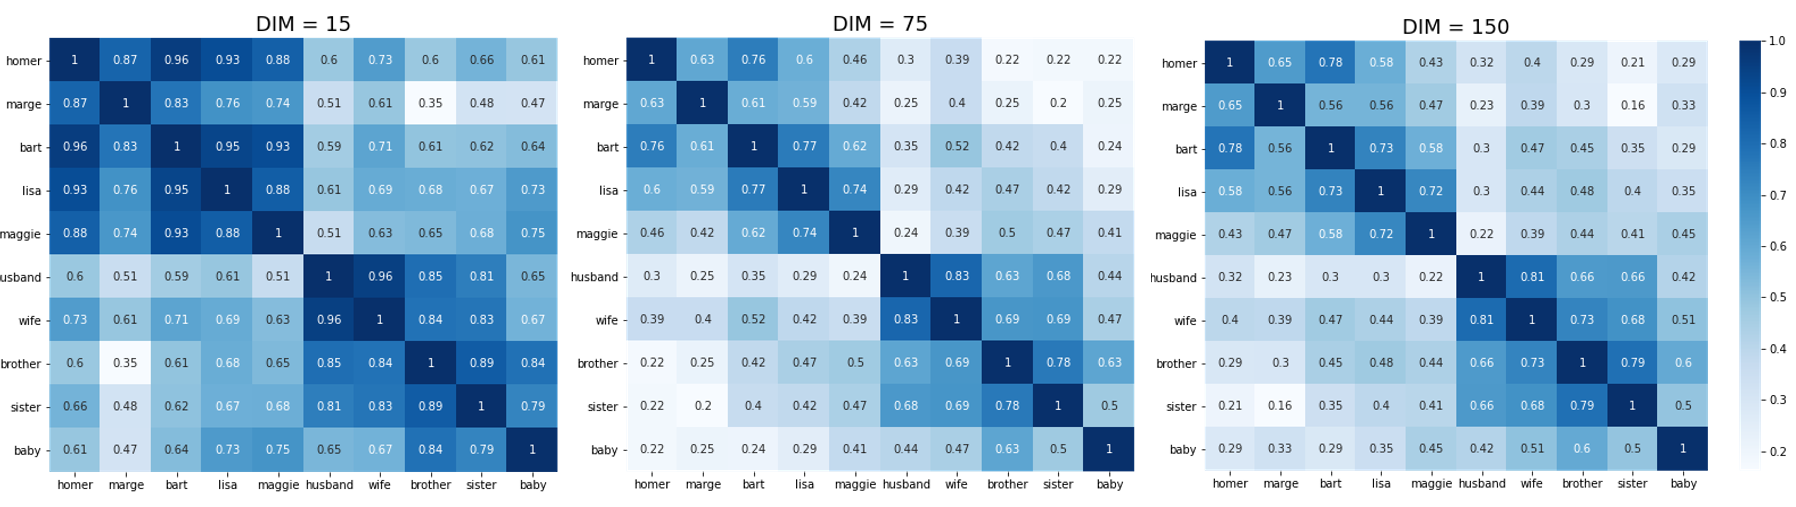
\includegraphics[width=\textwidth]{doc/images/simpsons_sim_matrix.png}
    \caption{Matriz de similitud entre términos relevantes del \textit{dataset} de los Simpsons.}
    \label{fig:simpsons_sim_matrix}
\end{figure}

Adicionalmente, se puede observar algunas relaciones de similitudes entre los personajes principales: Homero es más cercano a Bart, Bart es más cercano a Lisa, mientras que Marge tiene una similitud bastante igual con todos los personajes. Esto concuerda de alguna manera con el hecho de que las aventuras e historias de los personajes tienden a tener estas parejas de protagonistas en sus episodios.  \\

Otra punto importante a destacar es el hecho de que para una mayor dimensionalidad de \textit{embedding} la similitud entre terminos disminuye considerablemente (tendencia que también se ve en el \textit{dataset} de Friends). Casi pareciera que los términos \textit{bart} y \textit{homer} son intercambiables en el \textit{embedding} de 15, mientras que su relación es mucho menor en las otras dos dimensiones de \textit{embedding}. \\

Por su parte, al momento de evaluar las analogías, las relaciones de los embeddings presentaron resultados bastante sensatos como que: \textit{sister} es a \textit{lisa} como \textit{\textbf{brother}} es a \textit{bart} y que \textit{husband} es a \textit{homer} como \textit{\textbf{wife}} es a \textit{marge} (la palabra en negrilla fue predicha por el modelo). Asimismo, al momento de evaluar que termino no coincidía (o era el menos similar) los resultados concordaron con las relaciones que tienen los personajes dentro de la serie. Las comparaciones completas se pueden evidenciar en el cuaderno \texttt{HW03\_Embeddings.ipynb}.

\subsubsection{Friends Dataset}

De forma análoga, la figura \ref{fig:friends_sim_matrix} presenta las similitudes entre todos los personajes principales de la serie Friends y algunas otras palabras relevantes. En esta se observa nuevamente que las similitudes más fuertes están entre los personajes y entre términos con semántica similar como \textit{husband, wife} y \textit{friend}. Sin embargo, se pueden evidenciar algunas relacuiones interesantes como la similitud  entre \textit{central} y \textit{coffee} (Central Perk es el nombre del café al que siempre van). Y \textit{friend} con \textit{husband} y \textit{wife}. \\

\begin{figure}[H]
    \centering
    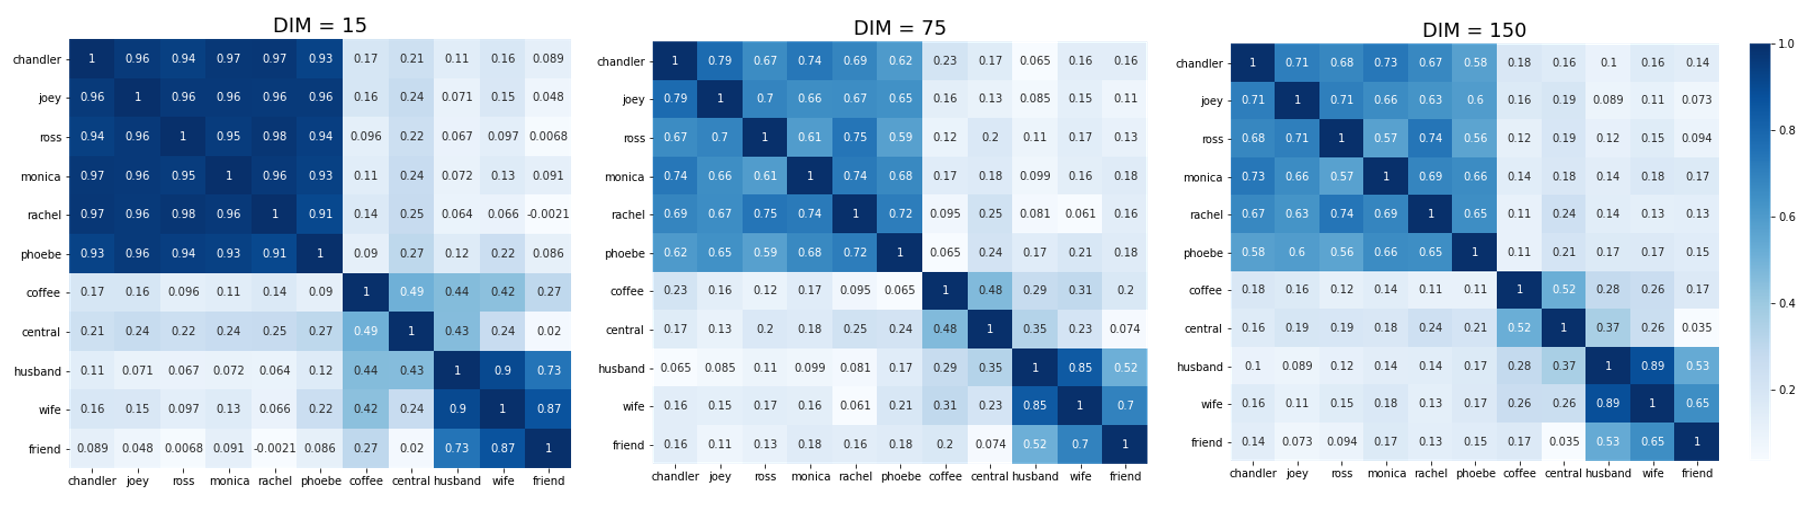
\includegraphics[width=\textwidth]{doc/images/friends_sim_matrix.png}
    \caption{Matriz de similitud entre términos relevantes del \textit{dataset} de Friends.}
    \label{fig:friends_sim_matrix}
\end{figure}

Adicionalmente, los personajes que sostienen una relación son aquellos que muestran una mayor cercanía, cómo lo son: \textit{Chandler y Monica} y \textit{Ross y Rachel}. 

\newpage